\documentclass[12pt,a4paper]{report}
\usepackage{cclicenses}
\usepackage{graphicx}
\title{Ceph Training Materials}
\author{Victor Denisov}
\date{\today}
\begin{document}
   \maketitle
\begin{abstract}
This work, ``Ceph Training Materials'', is derivative of ``Ceph Documentation'' http://docs.ceph.com/docs/master/ by Victor Denisov, used under \bysa. ``Ceph Documentation'' is licensed under \bysa by Inktank.
\end{abstract}

\chapter{Ceph Architecture}
Ceph uniquely delivers object, block, and file storage in one unified system.
Ceph is highly reliable, easy to manage, and free. Ceph delivers extraordinary
scalability–thousands of clients accessing petabytes to exabytes of data. A
Ceph Node leverages commodity hardware and intelligent daemons, and a Ceph
Storage Cluster accommodates large numbers of nodes, which communicate with
each other to replicate and redistribute data dynamically. All the components
of ceph storage cluster are presented on figure \ref{fig:ceph_architecture}

\begin{figure}[h]
	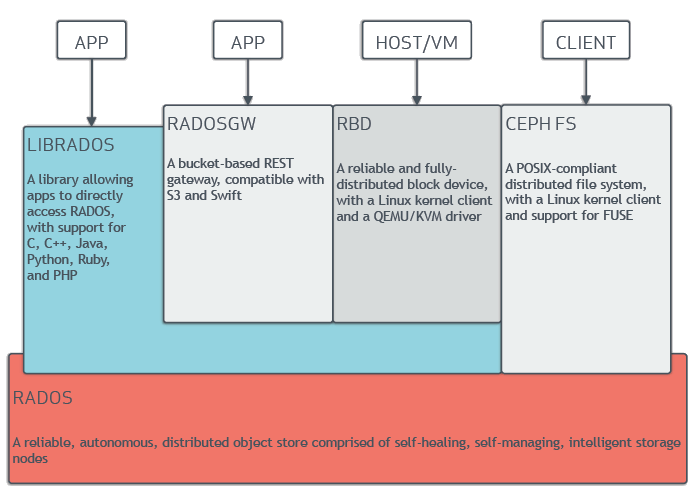
\includegraphics[scale=0.5]{stack.png}
	\caption{Ceph Architecture}
	\label{fig:ceph_architecture}
\end{figure}

\section{The Ceph Storage Cluster}
Ceph provides an infinitely scalable Ceph Storage Cluster based upon RADOS.
RADOS means Reliable Autonomic Distributed Object Store.

A Ceph Storage Cluster consists of two types of daemons:

\begin{itemize}
	\item Ceph Monitor
	\item Ceph OSD Daemon
\end{itemize}

A Ceph Monitor maintains a master copy of the cluster map. A cluster of Ceph
monitors ensures high availability should a monitor daemon fail. Storage
cluster clients retrieve a copy of the cluster map from the Ceph Monitor.

A Ceph OSD Daemon checks its own state and the state of other OSDs and reports
back to monitors.

Storage cluster clients and each Ceph OSD Daemon use the CRUSH algorithm to
efficiently compute information about data location, instead of having to
depend on a central lookup table. Ceph’s high-level features include providing
a native interface to the Ceph Storage Cluster via librados, and a number of
service interfaces built on top of librados.

\subsection{Storing Data}

The Ceph Storage Cluster receives data from Ceph Clients–whether it comes
through a Ceph Block Device, Ceph Object Storage, the Ceph Filesystem or a
custom implementation you create using librados–and it stores the data as
objects. Each object corresponds to a file in a filesystem, which is stored on
an Object Storage Device. Ceph OSD Daemons handle the read/write operations on
the storage disks.

\begin{figure}[h]
	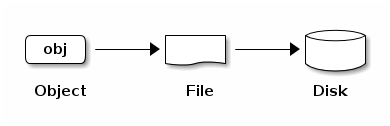
\includegraphics[scale=0.5]{object_file_disk.png}
	\label{fig:object_file_disk}
\end{figure}

Ceph OSD Daemons store all data as objects in a flat namespace (e.g., no
hierarchy of directories). An object has an identifier, binary data, and
metadata consisting of a set of name/value pairs. The semantics are completely
up to Ceph Clients. For example, CephFS uses metadata(figure
\ref{fig:object_metadata}) to store file attributes such as the file owner,
created date, last modified date, and so forth. Every object has an id which is
unique across the entire ceph cluster, not just the local filesystem.

\begin{figure}[h]
	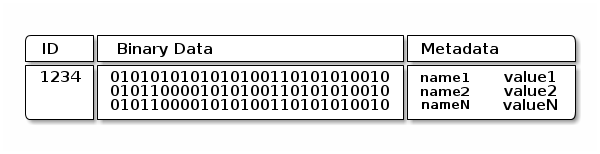
\includegraphics[scale=0.5]{object_metadata.png}
	\caption{Object's Metadata}
	\label{fig:object_metadata}
\end{figure}

\subsection{Scalability and High Availability}

In traditional architectures, clients talk to a centralized component (e.g., a
gateway, broker, API, facade, etc.), which acts as a single point of entry to a
complex subsystem. This imposes a limit to both performance and scalability,
while introducing a single point of failure (i.e., if the centralized component
goes down, the whole system goes down, too).

Ceph eliminates the centralized gateway to enable clients to interact with Ceph
OSD Daemons directly. Ceph OSD Daemons create object replicas on other Ceph
Nodes to ensure data safety and high availability. Ceph also uses a cluster of
monitors to ensure high availability. To eliminate centralization, Ceph uses an
algorithm called CRUSH.

\subsection{CRUSH Introduction}

Ceph Clients and Ceph OSD Daemons both use the CRUSH algorithm to efficiently
compute information about object location, instead of having to depend on a
central lookup table. CRUSH provides a better data management mechanism
compared to older approaches, and enables massive scale by cleanly distributing
the work to all the clients and OSD daemons in the cluster. CRUSH uses
intelligent data replication to ensure resiliency, which is better suited to
hyper-scale storage. The following sections provide additional details on how
CRUSH works. For a detailed discussion of CRUSH, see CRUSH - Controlled,
Scalable, Decentralized Placement of Replicated Data. \ref{crush_chapter}

\end{document}
